% --- LaTeX Homework Template - S. Venkatraman ---

% --- Set document class and font size ---

\documentclass[letterpaper, 11pt]{article}

% --- Package imports ---

\usepackage{
  amsmath, amsthm, amssymb, mathtools, dsfont,	  % Math typesetting
  graphicx, wrapfig, subfig, float,                  % Figures and graphics formatting
  listings, color, inconsolata, pythonhighlight,     % Code formatting
  fancyhdr, sectsty, hyperref, enumerate, enumitem } % Headers/footers, section fonts, links, lists
  
  \usepackage{tikz}
  
  \tikzset{
  vtx/.style={circle, fill=black, inner sep=1.6pt},
  every picture/.style={>=latex}
}

\usetikzlibrary{positioning}

% --- Page layout settings ---

% Set page margins
\usepackage[left=0.7in, right=0.7in, bottom=1in, top=1.1in, headsep=0.2in]{geometry}

% Anchor footnotes to the bottom of the page
\usepackage[bottom]{footmisc}



% Set line spacing
\renewcommand{\baselinestretch}{1.2}

% Set spacing between paragraphs
\setlength{\parskip}{1.5mm}

% Allow multi-line equations to break onto the next page
\allowdisplaybreaks

% Enumerated lists: make numbers flush left, with parentheses around them
\setlist[enumerate]{wide=0pt, leftmargin=21pt, labelwidth=0pt, align=left}
\setenumerate[1]{label={(\arabic*)}}

% --- Page formatting settings ---

% Set link colors for labeled items (blue) and citations (red)
\hypersetup{colorlinks=true, linkcolor=blue, citecolor=red}

% Make reference section title font smaller
\renewcommand{\refname}{\large\bf{References}}

% --- Settings for printing computer code ---

% Define colors for green text (comments), grey text (line numbers),
% and green frame around code
\definecolor{greenText}{rgb}{0.5, 0.7, 0.5}
\definecolor{greyText}{rgb}{0.5, 0.5, 0.5}
\definecolor{codeFrame}{rgb}{0.5, 0.7, 0.5}

% Define code settings
\lstdefinestyle{code} {
  frame=single, rulecolor=\color{codeFrame},            % Include a green frame around the code
  numbers=left,                                         % Include line numbers
  numbersep=8pt,                                        % Add space between line numbers and frame
  numberstyle=\tiny\color{greyText},                    % Line number font size (tiny) and color (grey)
  commentstyle=\color{greenText},                       % Put comments in green text
  basicstyle=\linespread{1.1}\ttfamily\footnotesize,    % Set code line spacing
  keywordstyle=\ttfamily\footnotesize,                  % No special formatting for keywords
  showstringspaces=false,                               % No marks for spaces
  xleftmargin=1.95em,                                   % Align code frame with main text
  framexleftmargin=1.6em,                               % Extend frame left margin to include line numbers
  breaklines=true,                                      % Wrap long lines of code
  postbreak=\mbox{\textcolor{greenText}{$\hookrightarrow$}\space} % Mark wrapped lines with an arrow
}

% Set all code listings to be styled with the above settings
\lstset{style=code}

% --- Math/Statistics commands ---

% Add a reference number to a single line of a multi-line equation
% Usage: "\numberthis\label{labelNameHere}" in an align or gather environment
\newcommand\numberthis{\addtocounter{equation}{1}\tag{\theequation}}

% Shortcut for bold text in math mode, e.g. $\b{X}$
\let\b\mathbf

% Shortcut for bold Greek letters, e.g. $\bg{\beta}$
\let\bg\boldsymbol

% Shortcut for calligraphic script, e.g. %\mc{M}$
\let\mc\mathcal

% \mathscr{(letter here)} is sometimes used to denote vector spaces
\usepackage[mathscr]{euscript}

% Convergence: right arrow with optional text on top
% E.g. $\converge[w]$ for weak convergence
\newcommand{\converge}[1][]{\xrightarrow{#1}}

% Normal distribution: arguments are the mean and variance
% E.g. $\normal{\mu}{\sigma}$
\newcommand{\normal}[2]{\mathcal{N}\left(#1,#2\right)}

% Uniform distribution: arguments are the left and right endpoints
% E.g. $\unif{0}{1}$
\newcommand{\unif}[2]{\text{Uniform}(#1,#2)}

% Independent and identically distributed random variables
% E.g. $ X_1,...,X_n \iid \normal{0}{1}$
\newcommand{\iid}{\stackrel{\smash{\text{iid}}}{\sim}}

% Equality: equals sign with optional text on top
% E.g. $X \equals[d] Y$ for equality in distribution
\newcommand{\equals}[1][]{\stackrel{\smash{#1}}{=}}

% Math mode symbols for common sets and spaces. Example usage: $\R$
\newcommand{\R}{\mathbb{R}}   % Real numbers
\newcommand{\C}{\mathbb{C}}   % Complex numbers
\newcommand{\Q}{\mathbb{Q}}   % Rational numbers
\newcommand{\Z}{\mathbb{Z}}   % Integers
\newcommand{\N}{\mathbb{N}}   % Natural numbers
\newcommand{\F}{\mathcal{F}}  % Calligraphic F for a sigma algebra
\newcommand{\El}{\mathcal{L}} % Calligraphic L, e.g. for L^p spaces

% Math mode symbols for probability
\newcommand{\pr}{\mathbb{P}}    % Probability measure
\newcommand{\E}{\mathbb{E}}     % Expectation, e.g. $\E(X)$
\newcommand{\var}{\text{Var}}   % Variance, e.g. $\var(X)$
\newcommand{\cov}{\text{Cov}}   % Covariance, e.g. $\cov(X,Y)$
\newcommand{\corr}{\text{Corr}} % Correlation, e.g. $\corr(X,Y)$
\newcommand{\B}{\mathcal{B}}    % Borel sigma-algebra

% Other miscellaneous symbols
\newcommand{\tth}{\text{th}}	% Non-italicized 'th', e.g. $n^\tth$
\newcommand{\Oh}{\mathcal{O}}	% Big-O notation, e.g. $\O(n)$
\newcommand{\1}{\mathds{1}}	% Indicator function, e.g. $\1_A$

% Additional commands for math mode
\DeclareMathOperator*{\argmax}{argmax}    % Argmax, e.g. $\argmax_{x\in[0,1]} f(x)$
\DeclareMathOperator*{\argmin}{argmin}    % Argmin, e.g. $\argmin_{x\in[0,1]} f(x)$
\DeclareMathOperator*{\spann}{Span}       % Span, e.g. $\spann\{X_1,...,X_n\}$
\DeclareMathOperator*{\bias}{Bias}        % Bias, e.g. $\bias(\hat\theta)$
\DeclareMathOperator*{\ran}{ran}          % Range of an operator, e.g. $\ran(T) 
\DeclareMathOperator*{\dv}{d\!}           % Non-italicized 'with respect to', e.g. $\int f(x) \dv x$
\DeclareMathOperator*{\diag}{diag}        % Diagonal of a matrix, e.g. $\diag(M)$
\DeclareMathOperator*{\trace}{trace}      % Trace of a matrix, e.g. $\trace(M)$

% Numbered theorem, lemma, etc. settings - e.g., a definition, lemma, and theorem appearing in that 
% order in Section 2 will be numbered Definition 2.1, Lemma 2.2, Theorem 2.3. 
% Example usage: \begin{theorem}[Name of theorem] Theorem statement \end{theorem}
\theoremstyle{definition}
\newtheorem{theorem}{Theorem}[section]
\newtheorem{proposition}[theorem]{Proposition}
\newtheorem{lemma}[theorem]{Lemma}
\newtheorem{corollary}[theorem]{Corollary}
\newtheorem{definition}[theorem]{Definition}
\newtheorem{example}[theorem]{Example}
\newtheorem{remark}[theorem]{Remark}

% Un-numbered theorem, lemma, etc. settings
% Example usage: \begin{lemma*}[Name of lemma] Lemma statement \end{lemma*}
\newtheorem*{theorem*}{Theorem}
\newtheorem*{proposition*}{Proposition}
\newtheorem*{lemma*}{Lemma}
\newtheorem*{corollary*}{Corollary}
\newtheorem*{definition*}{Definition}
\newtheorem*{example*}{Example}
\newtheorem*{remark*}{Remark}
\newtheorem*{claim}{Claim}
\newcommand{\Tau}{\mathcal{T}}
\newcommand{\PSet}{\mathcal{P}}





% --- Left/right header text (to appear on every page) ---

% Include a line underneath the header, no footer line
\pagestyle{fancy}
\renewcommand{\footrulewidth}{0pt}
\renewcommand{\headrulewidth}{0.4pt}

% Left header text: course name/assignment number
\lhead{MAM4000W, Graph Theory -- Chapter 4 Problems}

% Right header text: your name
\rhead{Alex Cristaudo, CRSALE010}

% --- Document starts here ---

\begin{document}

\subsection*{Question 1: Give an example of a planar graph in which no vertex has degree less than 5}

\begin{center}

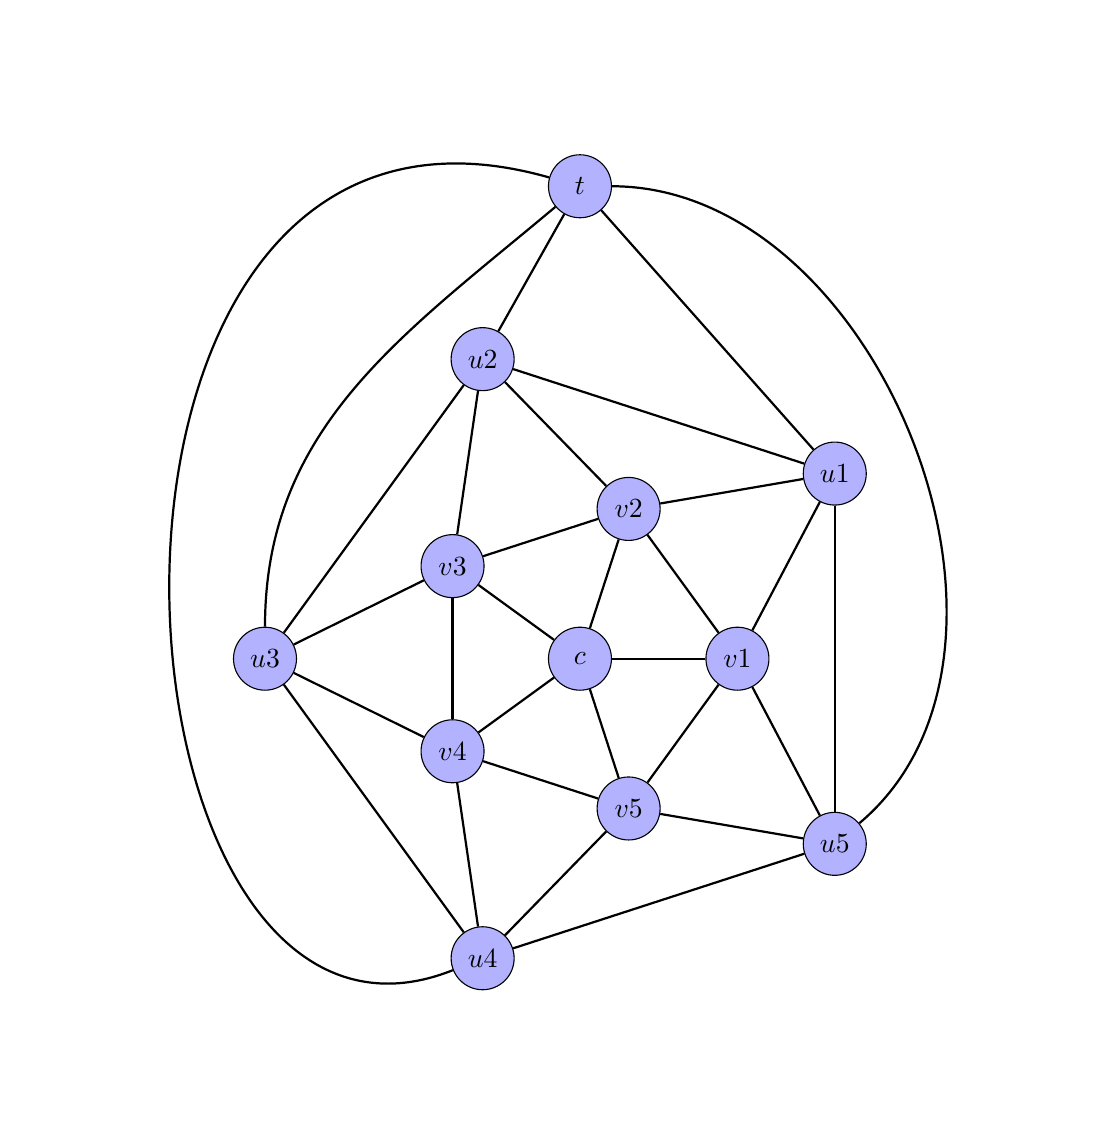
\begin{tikzpicture}[scale=2]

  % --- node style ---
  \tikzset{vtx/.style={circle, fill=blue!30, draw, minimum size=8mm, inner sep=0pt}}
  \tikzset{edge/.style={thick}}

  % inner pentagon
  \foreach \i in {1,...,5} {
    \node[vtx] (v\i) at ({cos(72*(\i-1))},{sin(72*(\i-1))}) {$v\i$};
  }

  % center vertex inside
  \node[vtx] (c) at (0,0) {$c$};

  % outer pentagon, rotated
  \foreach \i in {1,...,5} {
    \node[vtx] (u\i) at ({2*cos(72*(\i-1)+36)},{2*sin(72*(\i-1)+36)}) {$u\i$};
  }

  % apex outside
  \node[vtx] (t) at (0,3) {$t$};

  % --- edges ---
  % center to inner pentagon
  \foreach \i in {1,...,5} {
    \draw[edge] (c) -- (v\i);
  }

  % inner pentagon cycle
  \foreach \i/\j in {1/2,2/3,3/4,4/5,5/1} {
    \draw[edge] (v\i) -- (v\j);
  }

  % connect inner pentagon to outer pentagon (with slight curve)
%  \foreach \i in {1,...,5} {
%    \pgfmathtruncatemacro{\im}{mod(\i,5)+1} % i+1 mod 5
%    \draw[edge, bend left=15] (v\i) to (u\i);
%    \draw[edge, bend right=15] (v\i) to (u\im);
%  }

\draw[edge] (v3) -- (u3);
\draw[edge] (v3) -- (u2);
\draw[edge] (v4) -- (u3);
\draw[edge] (v4) -- (u4);
\draw[edge] (v5) -- (u4);
\draw[edge] (v5) -- (u5);
\draw[edge] (v1) -- (u5);
\draw[edge] (v1) -- (u1);
\draw[edge] (v2) -- (u1);
\draw[edge] (v2) -- (u2);

  % outer pentagon cycle
  \foreach \i/\j in {1/2,2/3,3/4,4/5,5/1} {
    \draw[edge] (u\i) -- (u\j);
  }

  % connect apex to all outer vertices with curves
%  \foreach \i in {1,...,5} {
%    \draw[edge, bend left=10] (t) to (u\i);
%  }


\draw[edge] (t) -- (u2);
\draw[edge] (t) -- (u1);
\draw[edge] (t) to[out=220,in=90] (u3);
\draw[edge] (t) to[out=0,in=40] (u5);
\draw[edge] (t) .. controls +(-3.5,1) and +(-2.5,-1) .. (u4);


\end{tikzpicture}

\end{center}

\subsection*{Question 2: If $G$ is a planar graph of order at least $4$, prove that $G$ contains at least four vertices of degree at most $5$}

We may assume that $G$ is maximal planar, since if there are at least 4 vertices of degree at most $5$ in $H$, a maximal planar extension of $G$, then the same applies for $G$. Let $N$ be the set of vertices of degree at most $5$. Then, \[
\sum \limits _{v \in V} \deg v = \sum \limits _{v \in N} \deg v + \sum \limits _{v\in V \setminus N} \deg v \ge |N| \cdot 3 + (n - |N|) \cdot 6 = 6n - 3|N|
\]
By the Handshaking Lemma, \[
\sum \limits _{v \in V} \deg v = 2m = 6n - 12
\]
So \[
6n - 12 \ge 6n - 3|N| \iff |N| \ge 4
\]
as required.

\subsection*{Question 3: Prove that there exists only one 4-regular maximal planar graph}
Suppose $G$ is a 4-regular maximal planar graph with order $n$. Then every vertex has degree $4$, so, by the Handshaking Lemma, $2m = 4n \iff m = 2n$. But since $G$ is maximal planar, we know $m = 3n - 6$. So we have that $3n - 6 = 2n \iff n = 6$. Take any vertex $v \in V(G)$ and let $N(u) = \{v_1,v_2,v_3,v_4\}$. Then, without loss of generality, there is a cycle $C: v_1,v_2,v_3,v_4,v_1$. Then there is one vertex $u \in V(G)$ such that $u \ne v$ and $u \notin N(v)$. Then, since $\deg u = 4$, and $u$ is not a neighbour to $v$, we must have that $uv_i \in E(G)$ for all $i \in \{1,2,3,4\}$ (all of $u$'s neighbours are the neighbours of $v$). This shows that $G$ must be unique, up to isomorphism, and is a graph looking as such:

\begin{figure}[h]
\centering
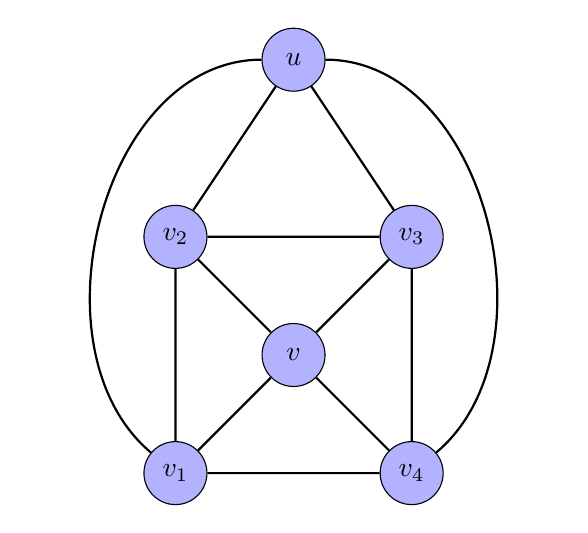
\begin{tikzpicture}[scale=1.5]
    \node[circle, fill=blue!30, draw, minimum size=8mm] (1) at (0,0) {$v_1$};
    \node[circle, fill=blue!30, draw, minimum size=8mm] (2) at (0, 2) {$v_2$};
    \node[circle, fill=blue!30, draw, minimum size=8mm] (3) at (2, 2) {$v_3$};
    \node[circle, fill=blue!30, draw, minimum size=8mm] (4) at (2, 0) {$v_4$};
    \node[circle, fill=blue!30, draw, minimum size=8mm] (5) at (1, 1) {$v$};
    \node[circle, fill=blue!30, draw, minimum size=8mm] (6) at (1,3.5) {$u$};

    
    \draw[thick] (1) -- (2) -- (3) -- (4) -- (1);
    \draw[thick] (1) -- (5) -- (3);
    \draw[thick] (2) -- (5) -- (4);
    \draw[thick] (6) -- (2);
    \draw[thick] (6) -- (3);
    \draw[thick] (6) to[out=180,in=140] (1);
    \draw[thick] (6) to[out=0,in=40] (4);
 
\end{tikzpicture}
\end{figure}

\subsection*{Question 4: Let $k \ge 3$ be an integer and let $G$ be a plane graph of order $n \ge k$ and size $m$ in which each cycle has length at least $k$.}

\subsubsection*{\ \ (a) Determine an upper bound $B$ for $m$ in terms of $n$ and $k$.}
Clearly $m \le 3n-6$. We use this bound if $G$ has no cycle (as otherwise $k$ can be any integer and our equation means nothing). If $G$ has a cycle, let $\epsilon (F)$ be the number of edges in $G[F]$. Then\[
\sum _F \epsilon (F) \le 2m
\]
(we might have bridges that only count an edge once). But for each face $F$, the number of edges in $G[F]$ is greater than $k$ (as these edges form a cycle). So $2m \ge fk$. By Euler's Formula, \[
2m \ge fk \iff 2m \ge (2 + m - n)k \iff 2m \ge 2k + mk - nk \iff m \le \frac{k}{k-2} (n-2)
\]
Since $m$ is an integer, we can further reduce this to \[
m \le \left \lfloor \frac{k}{k-2} (n-2) \right \rfloor
\]
(this upper bound is better because $k \ge 3$)
\subsubsection*{\ \ (b) Show that the bound $B$ obtained in the previous question is sharp by determining, for arbitrary $k \ge 3$, a plane graph $G$ of order $n$ and size $m = B$ in which every cycle has length at least $k$.}

Consider graph $C_k$. Every cycle has length $k$ (as there is only one cycle), $n = m = k$. So our upper bound is \[
B = \left \lfloor \frac{k}{k-2}(k-2) \right \rfloor = k = m
\]
as required.

\subsection*{Question 5: If $G$ is a plane graph and $F$ is any face of $G$, prove that $G$ can be embedded in the plane in such a way that $F$ is the outer face.}
We prove this by induction on the number of faces. If $f=1$, then the result follows trivially as it is the external face. So assume that, for $f \ge 1$, this result holds and let $G$ be a graph with $f+1$ faces. Then $f+1 \ge 2$ and $G$ is not a tree. Let $C$ be the cycle in the boundary of the external face $f_1$. Let $e$ be an edge on $C$, and $f_2$ the face that combines with $f_1$ in $G - e$. $G-e$ has $f-1$ faces, so every face can be embedded as the outer face. Thus, every face in $G$ except $f_2$ can be embedded as the outer face. We thus need to show $f_2$ can be embedded as the outer face. Let $C'$ be the cycle bounding $f_2$, then write the cycle on the external of graph $G-e$ (so $C'$ contains $G-e$. This is then an embedding with $f_2$ as the external face, as required.

\subsection*{Question 6: Euler's Formula applies only to connected planar graphs. Generalize Euler's Formula so that it can be used with any planar graph}
Suppose $G$ is a planar graph with components $C_1, C_2, ..., C_N$. Each component $C_i$, as a subgraph, has $n_i - m_i + f_i = 2$ for $i \in \{1,2, ..., N\}$. But then in $G$, we have \begin{align*}
n_G & = \sum \limits _{i=1}^N n_i \\ m_G &=  \sum \limits _{i=1}^N m_i  \\ f_G & = \sum \limits _{i=1}^N f_i  - (N-1)
\end{align*}
Since in the faces, we count the outer face $N$ times (one for each component). So \[
n_G - m_G + f_G = \sum \limits _{i=1}^N (n_i - m_i + f_i) - (N-1) = 2N - N + 1 = N + 1
\]
So for a graph with $c$ components, $n - m + f = c + 1$

\subsection*{Question 7: A graph $G$ is called \textit{outerplanar} if there is an embedding of $G$ in the plane such that
every vertex of $G$ lies on the boundary of the outer face.}
\subsection*{\ \ (a): Prove that $G$ is outerplanar if and only if $G + K_1$ is planar.}
Clearly if $G$ is outerplanar, $G + K_1$ is planar (by simply adding in a vertex on the external plane and connecting with arcs to the cycle). So suppose that $G + K_1$ is planar and consider a plane embedding. If $G + K_1$ has 1 face, clearly $G$ is outerplanar. So let $C$ be the cycle on the boundary of the outer face. Let $u$ be the vertex in $K_1$. Then either $u$ is on $C$, or it lies inside the cycle. In both cases, since $u$ is adjacent to every vertex on $C$, it divides $C$ into triangles. Any other vertex in $G$ must lie in one of those triangles. Any vertex adjacent to both corners of the triangle can join the cycle. Any adjacent to only one, can be placed on the exterior of the cycle by that vertex. Any adjacent to none are disconnected without $u$ and can be placed anywhere on the exterior. Removing $u$ gives us this result. We make the same argument for $u$ on the exterior. This shows $G$ is outerplanar. 
\subsection*{\ \ (b): If $G$ is an outerplanar graph of order $n \ge 2$ and size $m$, prove that $m \le 2n - 3$}
By (a), if $G$ is outerplanar, $H = G + K_1$ is planar. Then $n_H \ge 3$, so $m_H \le 3n_H - 6$. But $m_H = m_G + n_G$ (adding an edge for every vertex in $G$), so $m_H \le 3n_H - 6 \iff m_G + n_G \le 3 (n_G + 1) - 6 \iff m_G \le 2n_G - 3$
\subsection*{\ \ (c): Prove that a graph is outerplanar if and only if it contains no subdivision of $K_4$ or $K_{2,3}$}
Suppose that $G$ contains a subdivision $H$ of $K_4$. Then $H + K_1 \subseteq G + K_1$ is a subdivision of $K_5$. That is, $G + K_1$ is not planar (Kuratowski's Theorem) and thus not outerplanar. Similarly, if $G$ contains a subdivision of $K_{2,3}$, then adding a vertex $v$, and connecting it to the bipartite set with 3 vertices, this new graph is a subgraph of $G + K_1$ with this new vertex being the $K_1$ vertex (and only taking some of the new edges). Thus $G + K_1$ is not planar and $G$ is not outerplanar. Now suppose that $G$ is not outerplanar. Then $G + K_1$ is not planar. So $G + K_1$ contains a subdivision of either $K_5$ or $K_{3,3}$. If the vertex from $K_1$ is in the subdivision, simply removing it if so, or just removing any vertex (and the connecting edges), we get a subdivision of either $K_4$ or $K_{2,3}$.

\subsection*{Question 8: For each $k \in \{1,2,3\}$, find a nonplanar graph with chromatic number $k$, or prove
that no such graph exists.}
For $k = 1$, a graph has chromatic number $1$ if it is a collection of isolated vertices. This is clearly planar. For $k = 2$, use graph $K_{3,3}$ which is non-planar and bipartite, so each partite set is a colour. For $k = 3$, start with graph $K_{3,3}$, and add one new vertex connecting to one vertex from each partite set. Call this vertex $v$. Colouring $v$ with colour 1 forces the two partite sets to have different colours, both not 1. So 3 colours are needed as required.

\subsection*{Question 9: Recall that the average distance of a connected graph $G$ is $\mu (G) = \frac{2}{n(n-1)} \sum \limits _{u,v \in V(G)} d(u,v).$ If $G$ is a maximal planar graph of order $n$ and diameter $2$, find a formula for $\mu (G)$}

Suppose $G$ is of size $m$. Since $\text{diam}(G) = 2$, we have that $d(u,v) = 1$ or $d(u,v) = 2$ for $u \ne v$. We have that $u=v$ if and only if $d(u,v) = 0$, and $d(u,v) = 1$ if and only if graph $G$ has edge $uv \in E(G)$ . All other pairs of distinct vertices then have distance 2, with the total number of pairs of vertices being $\begin{pmatrix} n \\ 2 \end{pmatrix} = \frac{n(n-1)}{2}$. So \[
\sum \limits _{u,v \in V(G)}d(u,v) = 1 \cdot m + 2 \cdot \left (\frac{n(n-1)}{2} - m \right )
\]
Since $G$ is maximal planar, we have that $m = 3n-6$ and so \[
\mu (G) = \frac{2}{n(n-1)} \sum \limits _{u,v \in V(G)} d(u,v) = \frac{2}{n(n-1)} \left [ m + n(n-1) - 2m \right ] = \frac{2n(n-1) - 2m}{n(n-1)} = \frac{2n(n-1) - 2(3n - 6)}{n(n-1)}
\]
which simplifies to \[
\mu (G) = \frac{2n^2 - 8n + 12}{n(n-1)}
\]

\subsection*{Question 10: Not Applicable}
\subsection*{Question 11: If $G$ is a 2-connected plane graph, prove that the boundary of every face is a cycle.}
Assume that we have a face whose boundary is not a cycle. If $G$ contains no cycles, it is a tree and thus has bridges, a contradiction. So the boundary of this face contains a cycle, and an edge not on the cycle. Call this edge $e$. Then $e$ is a bridge (if $e = uv$, there is no other way for $u$ to reach $v$ other than edge $e$, otherwise we have another cycle and the boundary of our original face is a cycle), which contradicts that $G$ is 2-connected.

\subsection*{Question 12: Suppose that $G$ is a plane graph in which there are two regions with the same
boundary. Prove that G is a cycle.}
Let $F_1$ and $F_2$ be faces with the same boundary. Every edge lies in this common boundary lies between $F_1$ and $F_2$. Every edge can only separate exactly 2 faces. If we had more than 2 faces, at least 3, there would be an interior edge on the boundary of 2 faces, so they cannot have the same boundary as the external face. By considering the boundary of the external face, we can find an edge on the boundary of one face that isnt on the other. So we have exactly 2 faces, and let the boundary embedding be its largest cycle (possibly with other edges). If there are other edges on the cycle, they are either internal or external (in the cycle or outside). Internal implies that the internal faces boundary includes the edge but not the external face. Similarly, external gives a contradiction. Thus the boundary must just be a cycle.

\subsection*{Question 13: Prove Lemma 4.2.1}
Let $G$ be a maximal plane graph of order at least 3 and $F$ a face of $G$. Consider $G[F]$. The boundary contains some cycle $C_k$. Let $C_k$ be the cycle contained in the boundary for the smallest possible $k$. If $k \ge 4$, then we can find vertices $x$ and $y$ on the cycle $C_k$ with $xy \notin E(G)$. Adding edge $xy$ will not break planarity, as if it did, it must intersect another edge internal to our cycle and this would contradict that $C_k$ is the minimal cycle. But since we can add this edge, it contradicts that $G$ is maximal planar. So $G[F] \cong C_3$. From this, if $xy, xz \in E(G[F])$, then since $G[F] \cong C_3$, we must then have $yz \in E(G[F])$

\subsection*{Question 14: Prove that the average degree of the vertices of a planar graph is less than 6}
The average degree of a graph $G$ is given by: \[
\frac{\sum \limits _{v \in V(G)}\deg v}{n}
\]
By the Handshaking Lemma, $\sum \limits _{v \in V} \deg v = 2m$. If $n \ge 3$, then using that $m \le 3n - 6$ for planar graphs, we get\[
\frac{\sum \limits _{v \in V(G)}\deg v}{n} = \frac{2m}{n} \le \frac{6n - 12}{n} < \frac{6n}{n} = 6
\]
On the other hand, if $n < 3$, then $n = 1$ or $n=2$. Both cases are trivial, as the degree of each vertex cannot exceed 1

\subsection*{Question 15: Prove that every 5-connected planar graph has at least 12 vertices.}
In a planar graph, $\delta (G) \le 5$. But $\kappa (G) \ge 5$, by Witney's Theorem, implies $\delta (G) = 5$. Using the Handshaking Lemma, \[
6n - 12 \ge 2m = \sum \limits _{v \in V} \deg v \ge 5 n \Rightarrow n \ge 12
\]

\subsection*{Question 16: If $G$ is a planar graph and $S$ a triangle in $G$ (i.e., a subgraph isomorphic to $K_3$)
that is a vertex-cut, then $S$ is called a \textit{separating triangle}. Prove that a minimum
counterexample to the Four Colour Theorem cannot contain a separating triangle.}
(This questions works for the minimum with respect to $n$,$m$ or $f$, we will use $f$). Let $G$ be a counterexample to the Four Colour Theorem with minimal faces. Suppose that $G$ has a separating triangle $S$. Then $G - S$ has $\le f-1$ faces (as it splits into at least 2 components, removing a face and possible merging of faces). So we can colour $G-S$ with 4 colours.  But, since $S \cong K_3$, there are at most 3 faces adjacent to $S$ in $G$. This means we can colour $G$ with 4 colours (by simply using the colour not used in $G-S$), a contradiction. Thus any minimum counterexample to the Four Colour Theorem cannot contain a separating triangle.
~\\~\\ Doing it in terms of vertex-colourings, let $T$ be a separating triangle. Each component in $G - T$ can be coloured with 4 colours. Let $T = \{v_1,v_2,v_3\}$. Since we assume $G$ is minimal, $G - \{v_1\}$ is 4-colourable. So adding $v_2,v_3$ is 4-colourable. But the component that $v_1$ connects to is 4-colourable, and $G - v_2$ is also 4-colourable. So we can simply (possibly relabelling colours) colour $v_1$ in a new way
\subsection*{Question 17: Prove that ‘Every planar graph is 4-colourable’ and ‘Every maximal planar graph
is 4-colourable’ are equivalent statements (this implies that we may assume that a
minimum counterexample to the Four Colour Theorem is a maximal planar graph).}
(Note that this is vertex colouring, as a face colouring can be seen as a vertex colouring of a different graph, where the vertices are the faces and the edges are between faces that share a boundary)~\\
Since every maximal planar graph is itself a planar graph, we get that 'Every planar graph is 4-colourable' implies 'Every maximal planar graph is 4-colourable'. On the other hand, if every maximal planar graph is 4-colourable, then every planar graph can be extended to a maximal planar graph and will thus be 4-colourable as a subgraph of a 4-colourable graph.
\subsection*{Question 18: If $G$ is a maximal planar graph with $\delta (G) = 3$, prove that $G$ contains $K_4$ as a subgraph}

Since $G$ is maximal planar, we get $3 \le \kappa (G) \le \delta (G) = 3$. So $\kappa (G) = 3$. Let vertex $v$ be of minimal degree, so $\deg v = 3$. Then $|N(v)| = 3$, and so $N(u)$ is a minimal separating set. Then $\delta (G[N(u)]) \ge 2$ and it must follow that $\delta (G[N(u)]) = 2$, so $G[N(u)] \cong K_3$. But then the subgraph $G[N[u]] \cong K_4$, as every vertex has degree $3$.
~\\~\\ Or use the cycle $C(v)$ such that $V(C) = N(v)$

\subsection*{Question 19: Determine for which values of $t$ the hypercube $Q_t$ is planar.}
It is easy to show $Q_t$ is planar for $t=1,2,3$. We will show that $Q_4$ is not planar, and thus $Q_t$ is not for $t \ge 4$ as it contains $Q_4$ as a subgraph. We can characterise $Q_4$ as the graph of all binary strings of length $4$, and edges between vertices are those binary strings whose bits differ at exactly one position. We will find a subgraph of $Q_4$ that is a subdivision of $K_{3,3}$. Take vertex $(0,0,0,0)$ and edges to vertices $(0,0,0,1), (0,0,1,0), (0,1,0,0)$. Then take vertex $(1,0,0,0)$ and paths $(1,0,0,0) \to (1,1,0,0) \to (0,1,0,0)$, $(1,0,0,0) \to (1,0,1,0) \to (0,0,1,0)$, $(1,0,0,0) \to (1,0,0,1) \to (0,0,0,1)$, and finally vertex $(0,0,1,1)$ and paths $(0,0,1,1) \to (0,0,1,0)$, $(0,0,1,1) \to (0,0,0,1)$, $(0,0,1,1) \to (0,1,1,1) \to (0,1,0,1) \to (0,1,0,0)$. This subgraph is a subdivision of $K_{3,3}$ as required, so by Kuratowski's Theorem, it is nonplanar.

\subsection*{Question 20: Prove Corollary 4.3.2.}
(Rough sketch), Use the Art Gallery Theorem to get a collection of vertices and move them all slightly inwards, by some small $\varepsilon > 0$. The direction of moving can be taken as half the angle of the two vertices adjacent to the original vertex, directed inwards.

\subsection*{Question 21:}
N/A

\end{document}
